%% TODO: standardize use of "paramter" vs "system parameter" language
\section{Robustness to Static Parameter Deviations \label{sec:static}}
We have formulated the quantum optimal control
problem as an open loop optimization problem, i.e.
feedback from the experiment is not incorporated in optimization.
However, the device typically deviates from the Hamiltonian we use in optimization,
leading to poor experimental performance. We combat errors
of this form using robust control techniques,
making the state evolution insensitive
to Hamiltonian parameter deviations. As an example
we mitigate errors arising from the drift and finite measurement
precision of the qubit frequency $\tilde{f_{q}} = f_{q} \pm \sigma_{f_{q}}$.
We consider three robust control techniques.
The first is the sampling method, which has
been proposed previously in the context of QOC
\cite{rembold2020introduction, reinhold2019controlling, carvalho2020error}. In the
sampling method, multiple states are evolved under distinct deviant dynamics
to capture the effect of parameter deviations. We also
study the unscented sampling method, which uses the unscented
transformation to accurately propagate a distribution
representing the uncertainty in an evolving state
due to a parameter deviation.
The unscented transformation was designed for nonlinear Kalman
filtering and is frequently utilized in robust control
\cite{julier2004unscented, lee2013sigma, manchester2016derivative}.
Finally, we propose the derivative method. Derivative
information encoding the sensitivity of the
state trajectory with respect to the deviant parameter
is used to penalize state trajectory deviations.

In the sampling method, sample states evolve under a
Hamiltonian where a parameter is replaced by
a deviant value. We propagate the additional states $\ket{\psi^{\pm}}$ with
deviant values $\lambda^{\pm} = \lambda \pm \sigma_{\lambda}$.
The gate error of each sample state is 
penalized at each knot point
$1 - {\lvert \braket{\psi^{\pm}_{k} | \psi_{f}} \rvert}^{2}$.
Each initial state is used to initialize two
sample states $\ket{\psi^{\pm}}$.
The initial states are chosen so
that their outer products span the operators on the
Hilbert space $\{\ket{0}, \ket{1}, (\ket{0} + i\ket{1}) / \sqrt{2},
(\ket{0} - \ket{1}) / \sqrt{2}\}$ \cite{chow2009randomized}.
This is a standard perscription, though knowledge
of the problem can typically be used to reduced the number
of required samples. For this method the number of states in the augmented state vector
scales as $O(dn^{2})$ because each of $n^{2}$ initial
states is represented by $2d$ samples. $n$ is both the dimension of the Hilbert space
and the size of the state vector. $d$ is the number of deviant parameters.

%% F3
\begin{figure*}[ht]
  \begin{subfigure}{.4\textwidth}
    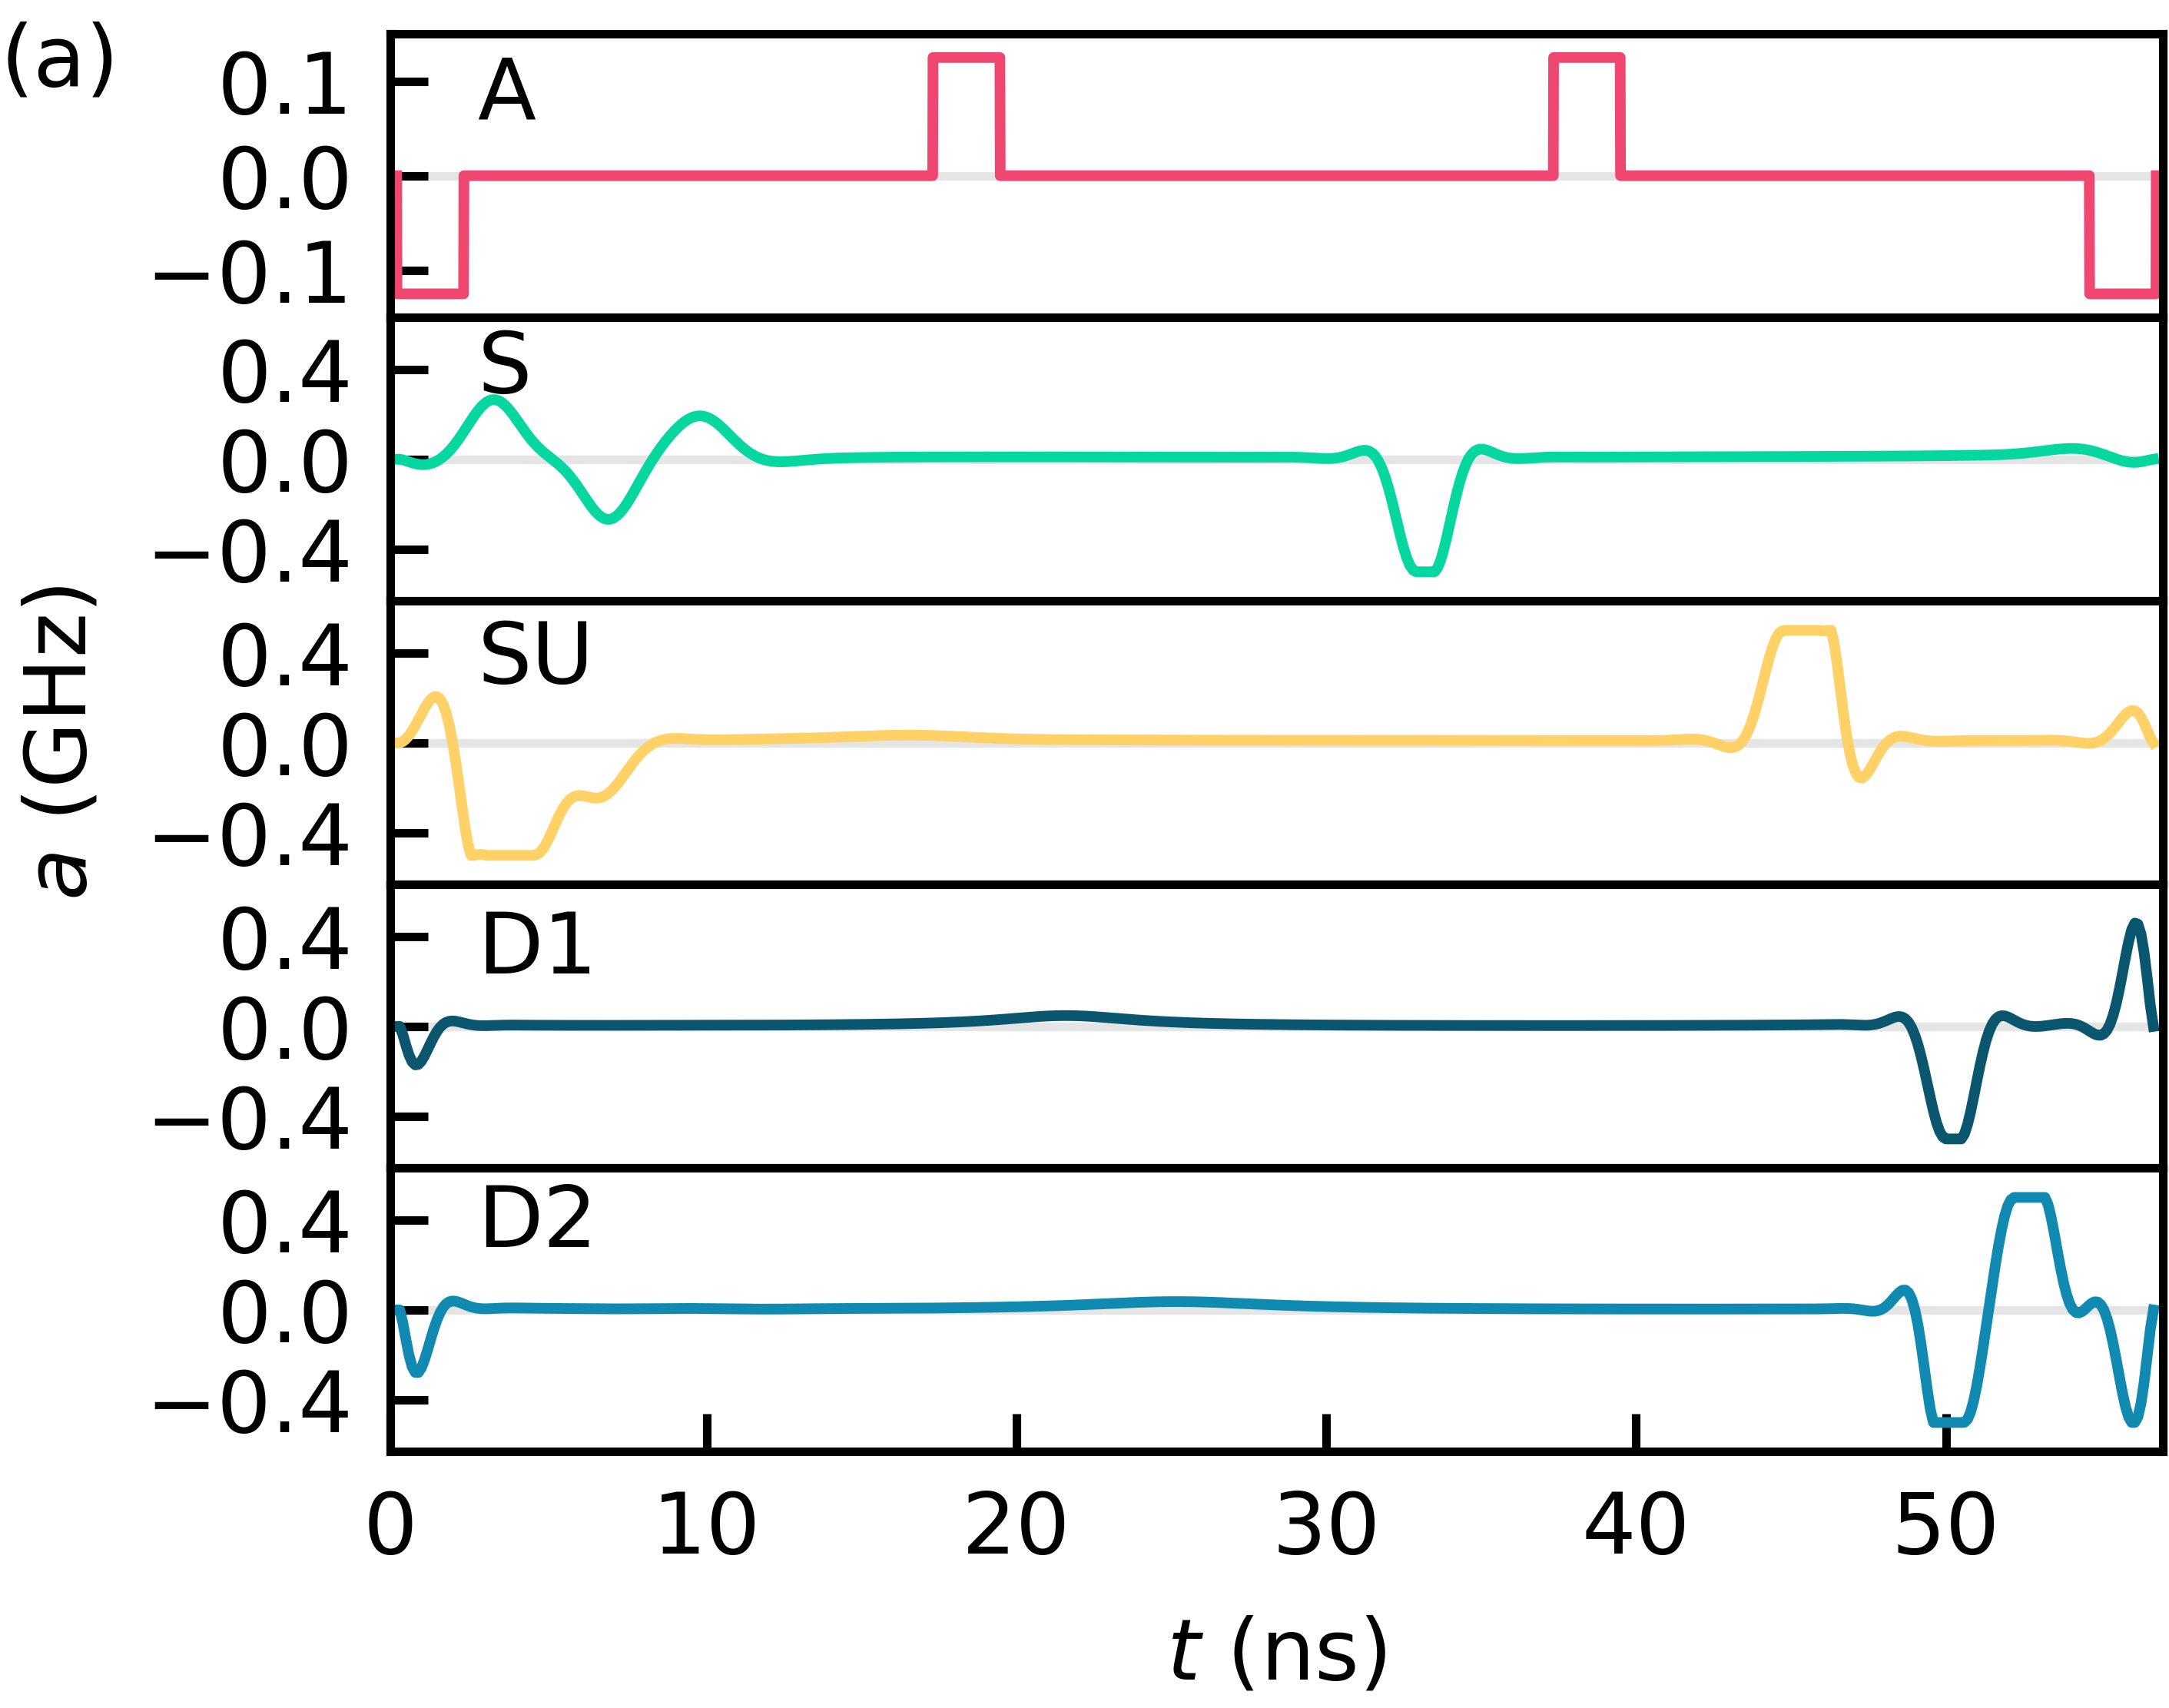
\includegraphics[width=\linewidth]{assets/f3a.png}
  \end{subfigure}\hspace{0.025\textwidth}
  \begin{subfigure}{.4\textwidth}
    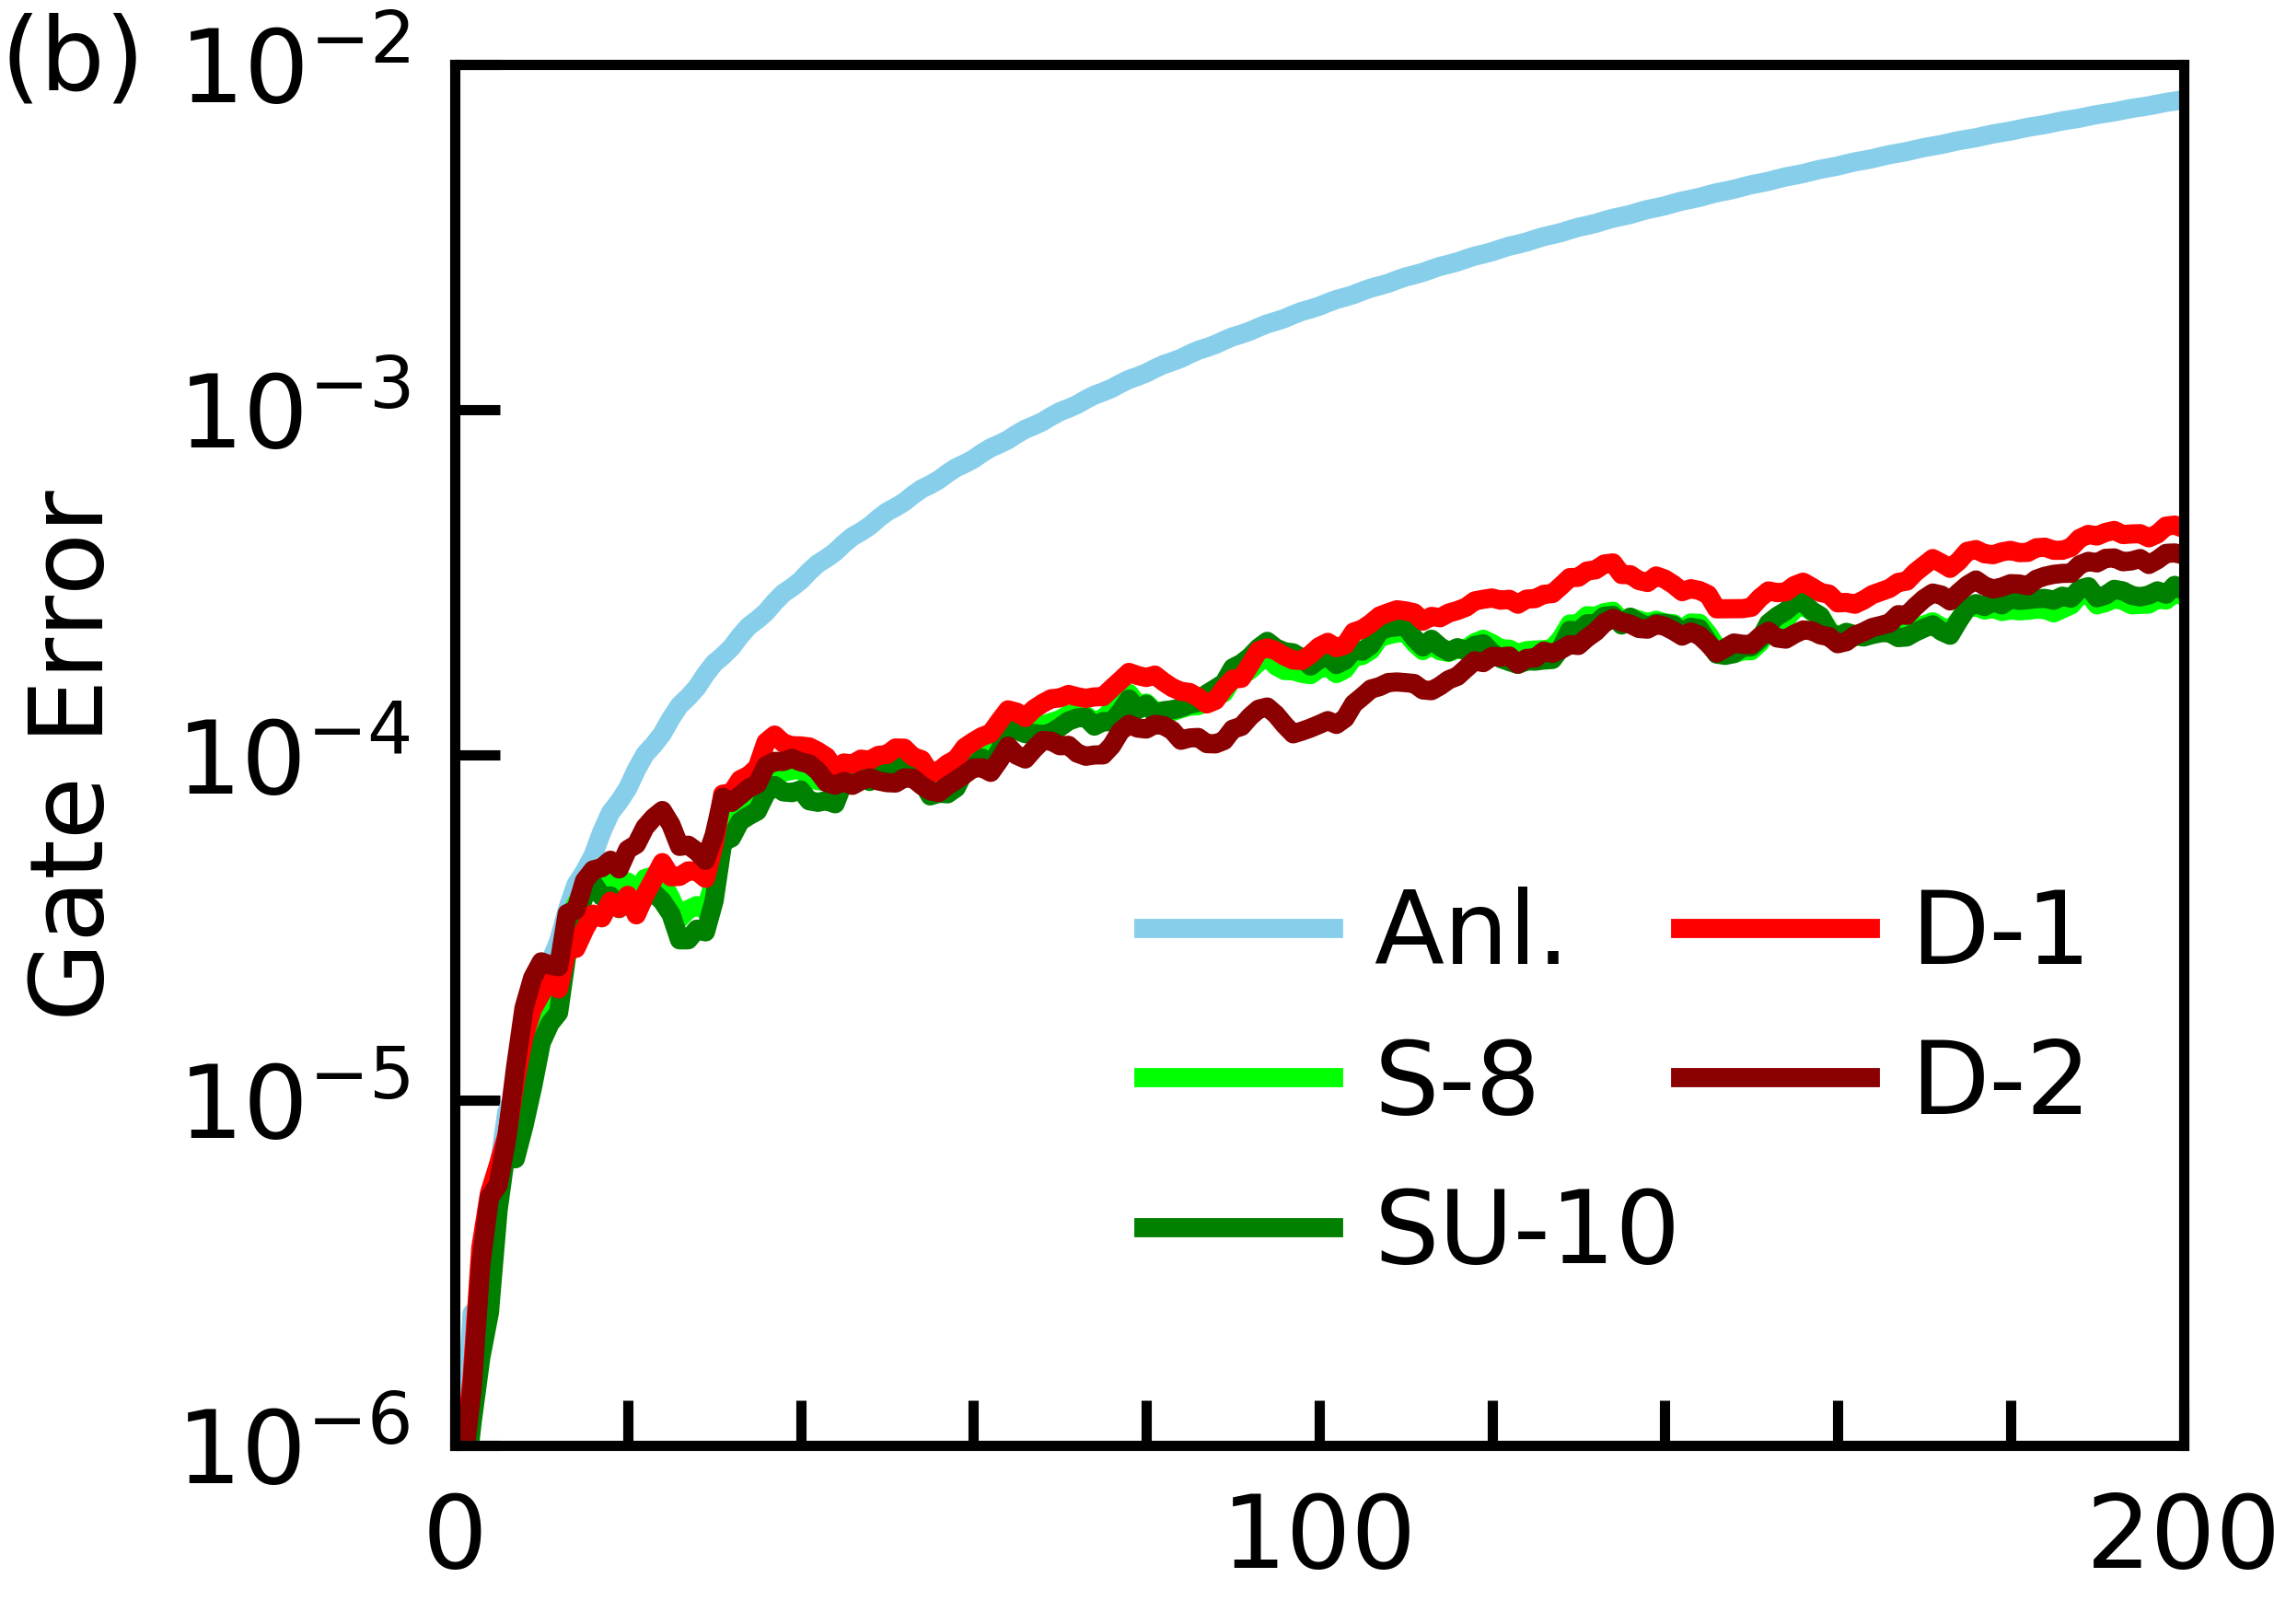
\includegraphics[width=\linewidth]{assets/f3b.png}
  \end{subfigure}
  \caption{
    (a) $X/2$ gates robust to flux offsets constructed with the analytic,
    sampling, unscented sampling, and the 1\textsuperscript{st}-
    and 2\textsuperscript{nd}-order derivative methods. The gates shown
    are the solutions at the analytic gate time.
    (b) Simulation of stochastic 1/$f$ flux noise for
    successive gate applications. The reported gate error is the cumulative
    gate error after each gate application.
  }
  \label{fig:stochastic}
\end{figure*}

The strategy of the unscented sampling method is to
propagate an ensemble of sample states (sigma points) which represent a distribution
over every element of the initial state. The distribution
models the uncertainty in each state element arising from the
parameter deviation. The ensemble consists of $4n + 2d$ states.
Each state in the
ensemble is propagated to the next
knot point using separate deviant dynamics. Then, the mean and covariance of
the propagated ensemble is calculated. New states are sampled from the distribution
given by the calculated statistics for propagation to the next knot point.
This resampling procedure, the unscented transformation, accurately propagates
first and second moments of the distribution and ensurnes the points
lie on the $\sqrt{2n}$\textsuperscript{th}
covariance contour at each knot point. A detailed update procedure is given
in Appendix \ref{appendix:unscented}. Each initial state from the operator basis
is represented with a distribution of $4n + 2d$ samples. Hence,
the number of states in the augmented state vector scales as $O(n^{3} + dn^{2})$.
The gate error of each sample state is penalized as in the sampling method.

The derivative method draws on the intuition that
the sensitivity of the state evolution to a parameter
$\lambda$ is encoded in the $l$\textsuperscript{th}-order
derivative of the state with respect to that parameter
$\ket{\partial_{\lambda}^{l} \psi}$. The $m$\textsuperscript{th}-order
derivative method minimizes the norm of the first $m$
state derivatives with a quadratic cost at each knot point
${\lvert \braket{\partial^{l}_{\lambda} \psi | \partial^{l}_{\lambda} \psi}
  \rvert}^{2}$, $l \in \{1, \dots, m\}$.
The state derivatives could be obtained with backwards mode differentiation.
Naive automatic differentiation would compute
the state derivative at all $1, \dots, k - 1$ knot points
to obtain the state derivative at knot point $k$.
For a single state derivative and $N$ knot points this
requires $O(N^2)$ matrix multiplications.
Instead, we forward propagate the state derivatives in the
augmented state vector under coupled dynamics, resulting in
$O(N)$ matrix multiplications. For example, the dynamics
for the 1\textsuperscript{st}-order derivative method are
\begin{align}
  i \hbar \frac{d}{dt} \ket{\psi} &= H \ket{\psi}\\
  i \hbar \frac{d}{dt} \ket{\partial_{\lambda}\psi} &=
  H \ket{\partial_{\lambda} \psi} +
  (\partial_{\lambda} H) \ket{\psi}
\end{align}
Exponential integrators that account for the non-linear
term may be used to efficiently integrate the coupled dynamics,
see Appendix \ref{appendix:derivative}.
For this method $m$ state derivatives are associated with each
initial state from the operator basis.
So, the number of states in the augmented state vector scales as
$O(dmn^{2})$.

To demonstrate the applicability of these techniques
to mitigate system parameter deviations,
we consider the task of achieving a single $Z/2$
gate subject to a constant qubit frequency detuning
$f_{q} \gets f_{q} + \delta f_{q}$.
We take $\sigma_{f_{q}} / f_{q} = 1\%$ to be one standard devation, and equip
the sampling methods accordingly. For each method we compute the gate error for
one simulated gate application subject to the deviant dynamics given by the
stated qubit frequency detuning $\delta f_{q}$.

We compare the numerical methods
to an analytically derived $Z/2$ gate, see Figure \ref{fig:static}a. This gate corresponds to
idling at the flux frustration point $a = 0$. The analytic gate
is at the device's speed limit for a $Z/2$ gate $t_{Z/2} = 1 / 4 f_{q}$ and
is simple to derive. Its erroneous rotation angle $2 \pi t_{Z/2} \delta f_{q}$ is linearly sensitive to
the qubit frequency detuning, resulting in a gate error that is quadratically sensitive
to the qubit frequency detutning.
At a one-percent
qubit frequency detuning the analytic gate achieves a gate error $\sim 4.5 \cdot 10^{-5}$,
which is sufficient for quantum error correction, see Figure \ref{fig:static}b.
Although the analytic $Z/2$ gate performs well, it works
only at the gate time $t_{Z/2}$. The ability to perform $Z$ rotations in arbitrary times is critical
for operating multi-qubit experiments in the lab frame.
Each numerical method is able to find solutions at
all gate times above $t_{Z/2}$, but is unable to find solutions at shorter times.
These numerical methods offer an effective scheme for synchronizing
qubits operating at different frequencies $f_{q, i} \neq f_{q, j}$.

%% TOOD: intro sentence
%% TODO: comment on unscented when it is redone
The sampling and unscented sampling methods
converge on qualitatively similar solutions which combine idling periods
with fast ramps to the maximum amplitude. The gate error at a one-percent
detuning from the nominal qubit frequency achieved
by the sampling method does not improve substantially over the
range of gate durations. The unscented sampling method
achieves linear decreases in its gate error with longer gate durations
until half the larmor period $1 / 2 f_{q}$ after which it achieves a consistent
gate error $\sim 3.5 \cdot 10^{-5}$.
The derivative methods converge on qualitatively similar solutions that
use fast traingle pulses at the boundaries and balance time
on either side of the flux-frustration point symmetrically at low amplitudes.
Both methods achieve a super-linear scaling in their gate error as
a function of the gate duration. The gate error for the 1\textsuperscript{st}-order
derivative method approaches zero at the larmor period $1 / f_{q}$, see Figure \ref{fig:static}c.
We believe the 1\textsuperscript{st}-order method outperforms the 2\textsuperscript{nd}-order
method due to the low contribution of second-order
terms to the gate error in this deviation regime, see Appendix \ref{appendix:derivative}.


%% TODO: how do I tie this in?
Multiple analytic methods have also been presented to construct gates
that mitigate the error arising from parameter deviations
including composite pulse sequences \cite{merrill2014progress},
the DRAG scheme \cite{krantz2019quantum}, and
geometric phase considerations
\cite{xu2020nonadiabatic, han2020experimental}.
Composite pulse sequences are derived by computing
the erroneous rotation arising from the static parameter deviation
with a finite order magnus expansion.
Pulses are then suitably composed to eliminate the
error. In principle the error may be eliminated
to arbitrary order with sufficiently many pulses.
It is difficult to choose an appropriate composite pulse
for comparison on the problem we study here. We
propose comparing numerical methods to existing analytic
techniques for future work.
